\chapter{Simulations of the Artificial SMMF}\label{app:SMMF_sims}


\section{Model}

The artificial data used in the simulations of the SMMF was created using 2 very simplistic models, either separately or in combination, which are physically motivated by sunspots and active regions on the solar surface:

\begin{enumerate}
	
	\item{{\bf Cosine}: in this model a source was simulated as a single region which appears on the visible disk from one limb, traversing across the disk, before disappearing off the other limb (see Fig.~\ref{fig:cosine_model}). The physical motivation for this would be a single, concentrated source of imbalanced magnetic flux. This method induces no sign change of the simulated source; it remains the same polarity always. This was simulated as a rectified sinusoidal signal, with a 50$\%$ duty cycle (i.e. it is only visible during times on near-side of the disk).}
	
	\item{{\bf Sign change}: in this model a source was simulated as 2 regions of opposite polarity, such as sunspot pairs or bipolar magnetic regions (BMRs). The leading region contributes more at the start of the transit during ingress, and the trailing source contributes more at the end of the transit during egress; hence at the middle of the transit we assume there is a sign change in the overall signal, see Fig.~\ref{fig:sgn_cng_model}. This was simulated as a rectified sinusoidal signal, and was multiplied by a cosinusoidal signal of the same period to provide the projection of the pair of regions. This operation results in a rectified sinusoidal signal with half the period.}
	
\end{enumerate}

\begin{figure}
	\centering
	\subfloat[`cosine' model \label{fig:cosine_model}]{
\includegraphics[width=0.35\columnwidth]{cosine_model.pdf}} 
	\qquad
	\subfloat[`sign change' model \label{fig:sgn_cng_model}]{
\includegraphics[width=0.35\columnwidth]{sgn_cng_model.pdf}}
	\caption{Schematic representations of the two models of the artificial SMMF. (a) shows the cosine model with a single source of constant polarity transiting the visible disk. (b) shown the sign change model whereby there are 2 regions of opposite polarity transiting the disk, and their contribution to the SMMF changes during the transit.}  \label{fig:artificial_models}
\end{figure}


In the simulations there were several variables that allowed us to change the physics of the simulations. These were:

\begin{itemize}
	\item{{\bf $N$}: Number of sources}
	\item{{\bf $t_0$}: Start time of source appearance}
	\item{{\bf $A$}: Amplitude of sources}
	\item{{\bf $\lambda$}: Latitude of sources}
	\item{{\bf $\tau$}: Decay time of sources}
	\item{{\bf $\phi$}: Additional phase of sources}
\end{itemize}

Using these variables, the mathematical form of the simulation for a single source is expressed by equation~(\ref{eq:cosine_model}) and equation~(\ref{eq:sgn_cng_model}). In these equations $t' = t - t_0$, $\Pi_{P/2}(t)$ is a window function to define the transit period of the simulated source on the visible side of the solar disk, $\mathrm{III}_{P}$ is a Dirac comb of frequency, P, and $\Pi_{T}(t)$ is a window function defining the total observation period. The time series of a single modelled source for each model is shown in Figure~\ref{fig:artificial_models}.

\begin{equation}
B_{\mathrm{cosine}}(t) = \left[ A e^{-t'/\tau} \, \left( \cos{\left(\frac{2\pi}{P}t' + \phi\right)} \, \Pi_{P/2}(t) \right) * \mathrm{III}_{P} \right] \times \Pi_{T}(t)
\label{eq:cosine_model}
\end{equation}


\begin{equation}
B_{\mathrm{sign-change}}(t) = \left[ A e^{-t'/\tau} \, \left( \cos{\left(\frac{2\pi}{P}t' + \phi\right)} \, \sin{\left(\frac{2\pi}{P}t' + \phi\right)} \, \Pi_{P/2}(t) \right) * \mathrm{III}_{P} \right] \times \Pi_{T}(t)
\label{eq:sgn_cng_model}
\end{equation}


\begin{figure}[ht!]
	\centering
	\subfloat[`cosine' model \label{fig:cosine_TS}]{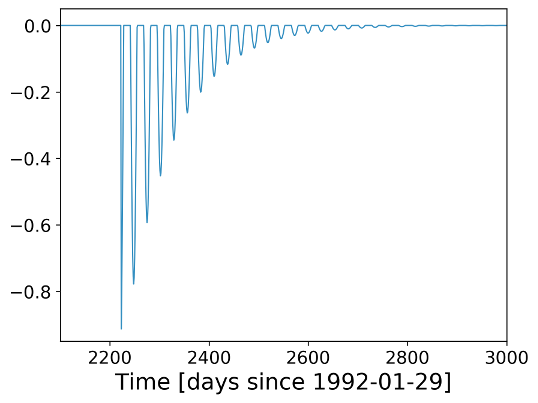
\includegraphics[width=0.45\columnwidth]{fake_TS_cosine_rescaled.png}} 
	\qquad
	\subfloat[`sign change' model \label{fig:sgn_cng_TS}]{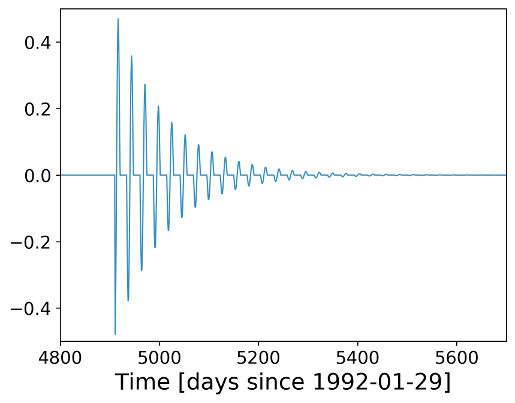
\includegraphics[width=0.45\columnwidth]{fake_TS_sgn_cng_rescaled.png}}
	\caption{A single realisation of (a) the cosine model, and (b) the sign change model.}  
	\label{fig:artificial_TS}
\end{figure}


\section{Configuration of the Simulations}

A flowchart describing the steps in the simulations is shown in Figure~\ref{fig:flowchart}. The simulations require the user to select the number of sources to be modelled. Using this information, the user selects whether to draw N seed/start times ($t_0$) from either a kernel density estimate (KDE) of the SSN, or from a uniform distribution between the start and end times. The former will give an output which is more physical, but the latter is useful for testing.

From the generated seed times, latitudes are computed using a model for the migration of spots during the Solar Cycle \citep{li_latitude_2001-1}, and the differential rotation frequency at that latitude is taken from a model of the solar differential rotation \citep{snodgrass_magnetic_1983}. 

Values are then assigned for the phase, amplitude, and decay time of each source (the user can set these parameters, or it is also possible to randomly select them from a distribution). Each individual source is then simulated according to equation~(\ref{eq:cosine_model}) or equation~(\ref{eq:sgn_cng_model}), and the full time-series is computed by adding all N sources together. Finally, a burn-in period is removed, which allows the artificial SMMF to settle prior to the start of `observations', and then we can inject gaps into the artificial time series which are concurrent with the gaps in the BiSON observations.


\begin{figure}[ht!]
	\centering
	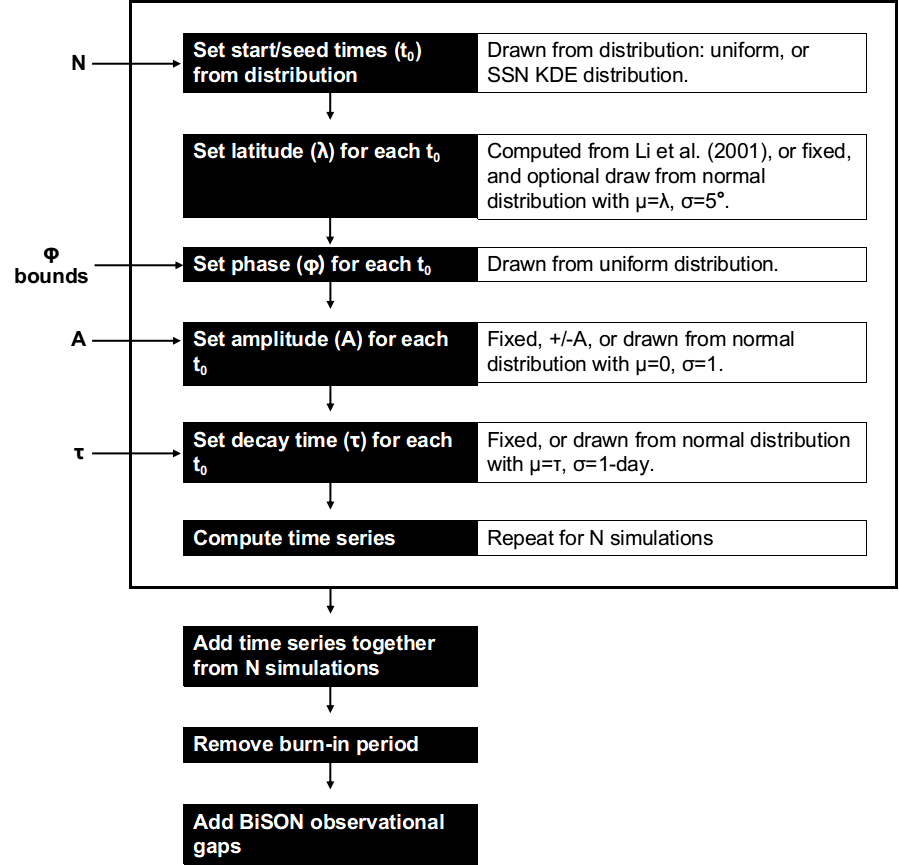
\includegraphics[width=0.85\columnwidth]{flow_chart_2.png}
	\caption{Flowchart showing the step-by-step processes in the generation of the artificial SMMF time series data.}
	\label{fig:flowchart}
\end{figure}


The aim of creating artificial data was to produce a representative power spectrum to that of the BiSON SMMF. We assume that the sources of the SMMF are active regions of magnetic flux, therefore we aimed to produce a time series that physically represented these sources, i.e. comparable to the sun spot number. To do this we produced an average number of sources on the visible disk during close to the sunspot number. At solar maximum during cycle 23, the number of daily spots on the disk is around 150 -- 200. 

Including a year for burn-in, such that the interferences between the sources stabilises (see Figure~\ref{fig:artificial_sim_burn-in}), we chose to select N~=~20000 and $\tau$~=~100 days, which produces a median total of $\sim$17450 sources over the BiSON observational epoch of 7633 days, with an average of around 150 -- 200 sources per day on the visible disk during solar cycle 23 maximum, as shown in Figure~\ref{fig:artificial_sim_config}.


\begin{figure}[!ht]
	\centering
	\subfloat[Burn-in]{
		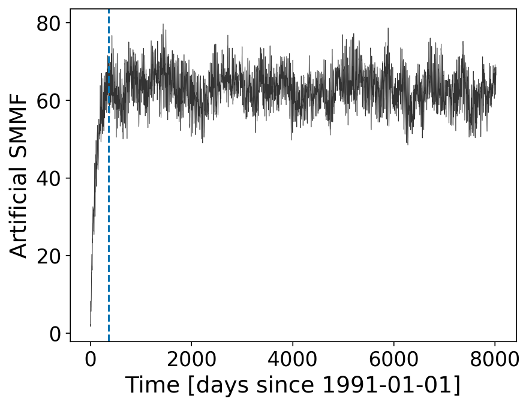
\includegraphics[width=0.45\columnwidth]{burn-in_TS_rescaled.png}
		\label{fig:artificial_sim_burn-in}}
	\qquad
	\subfloat[Number of sources in the simulation after burn-in]{
		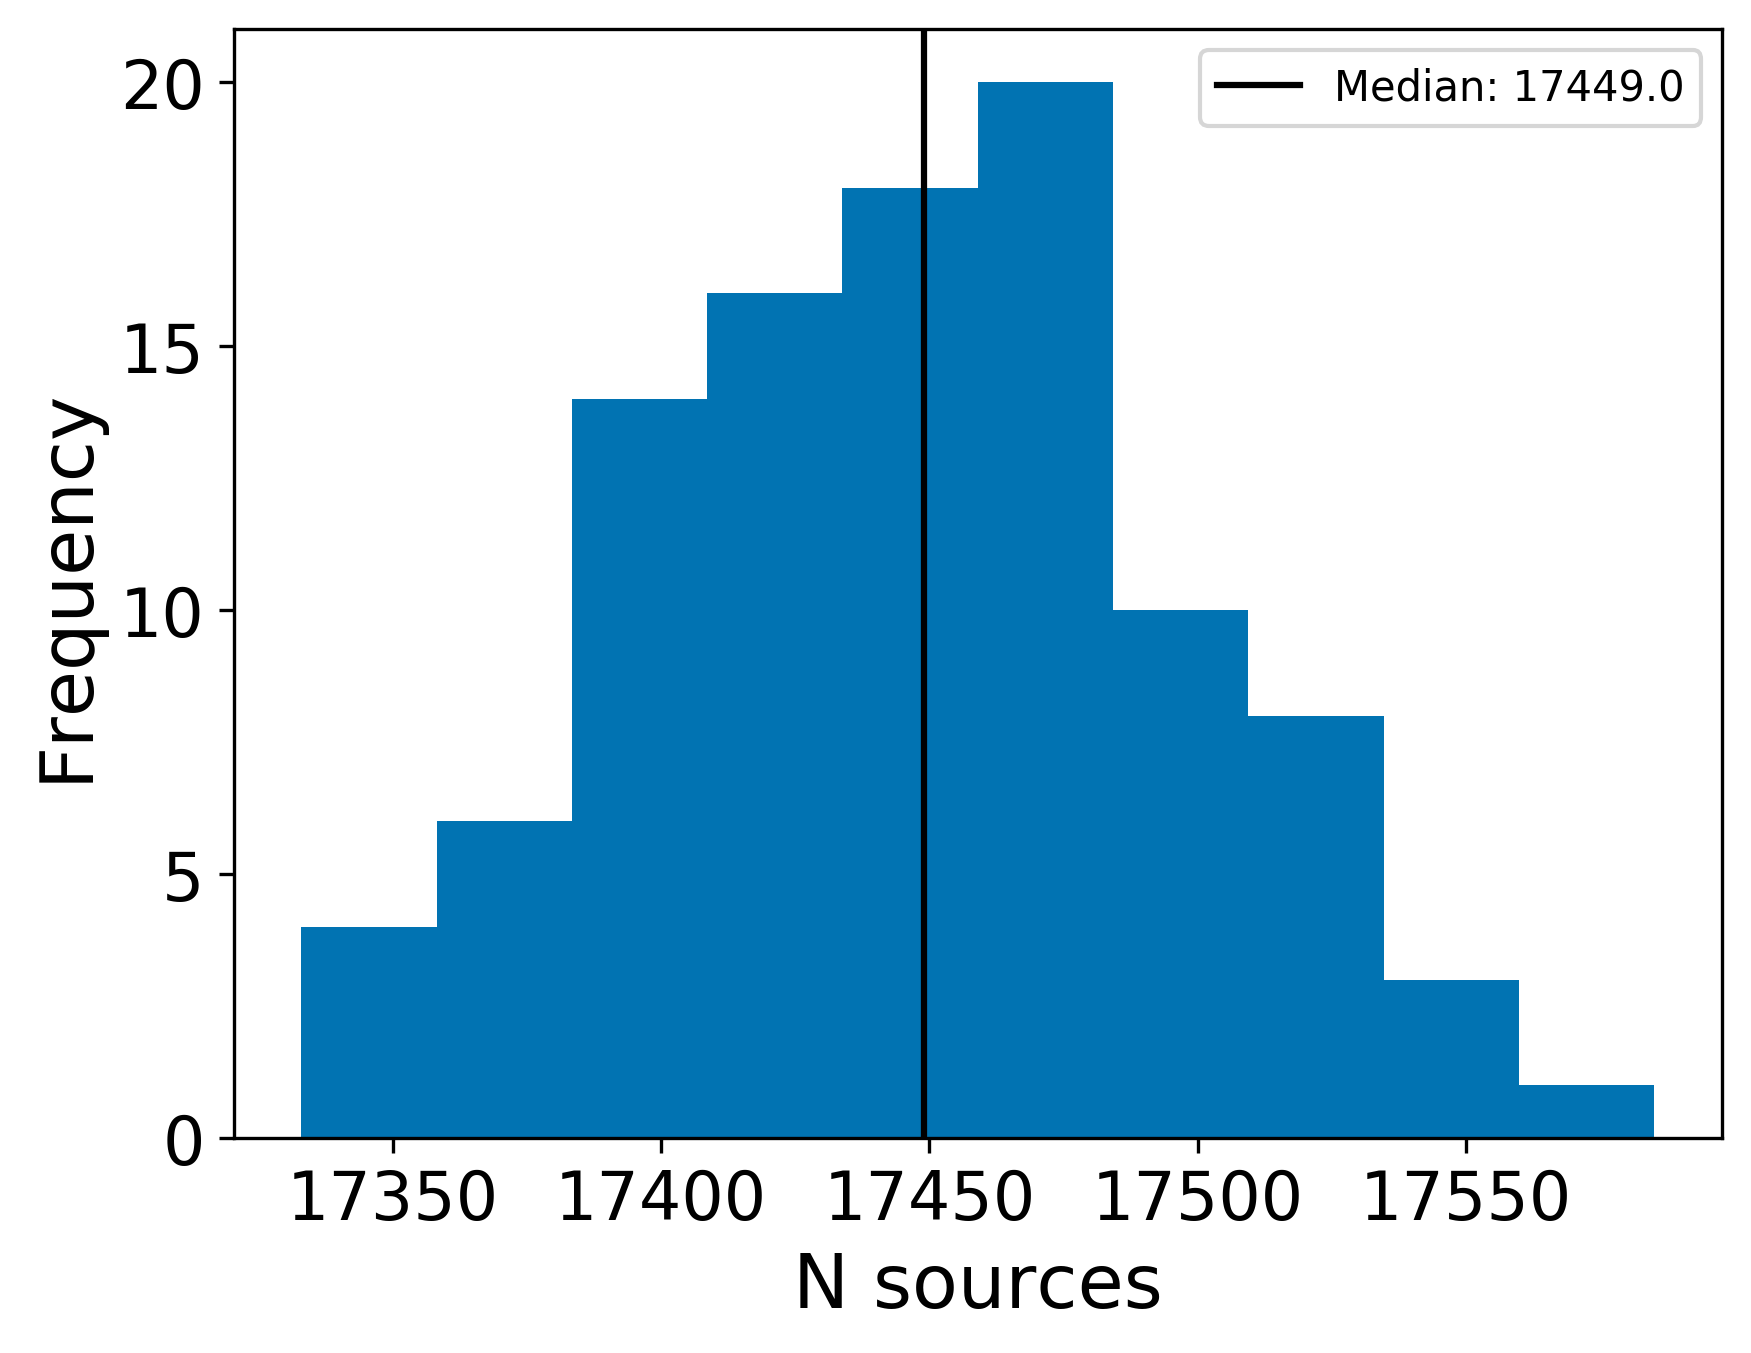
\includegraphics[width=0.45\columnwidth]{N_hist.png}
		\label{fig:artificial_sim_N}} \\
	
	\qquad
	
	\subfloat[Sources on the visible disk]{
		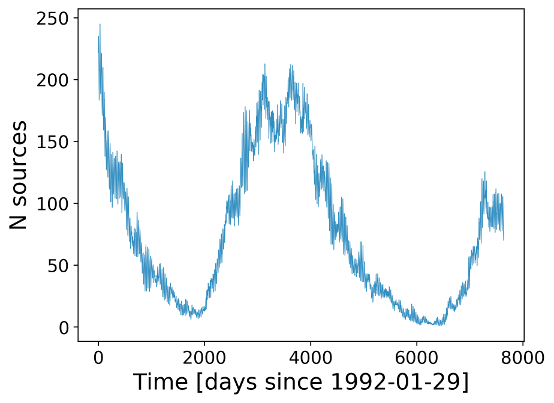
\includegraphics[width=0.45\columnwidth]{fake_sources_rescaled.png}
		\label{fig:artificial_sim_sources}}
	\qquad
	\subfloat[Sunspot number]{
		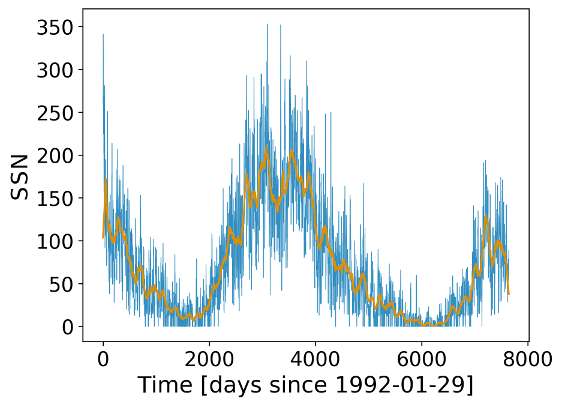
\includegraphics[width=0.45\columnwidth]{SSN_rescaled.png}
		\label{fig:artificial_sim_SSN}}
	
	\caption{(a) the burn-in period required to ensure that the interference of sources stabilises. (b) histogram of the number of sources which remain in the simulation (out of the 20000 input), after the burn-in is removed. (c) the number of simulated sources on the visible disk over the BiSON observational epoch. (d) the daily-averaged sunspot number (blue, and the monthly-averaged sunspot number (orange)).}
	\label{fig:artificial_sim_config}
\end{figure}


\section{Outputs}


The simulation produces the total time series data output from the combination of all sources, along with the Fourier transform of the time series. A butterfly diagram, from a realisation which allows for a more realistic, stochastic simulation, whereby the values for parameters are drawn from a distribution with scatter, is shown in Figure~\ref{fig:fake_butterfly}. This butterfly diagram shows a strong resemblance to a true, observational butterfly diagram of the Sun.


\begin{figure}[ht!]
	\centering
	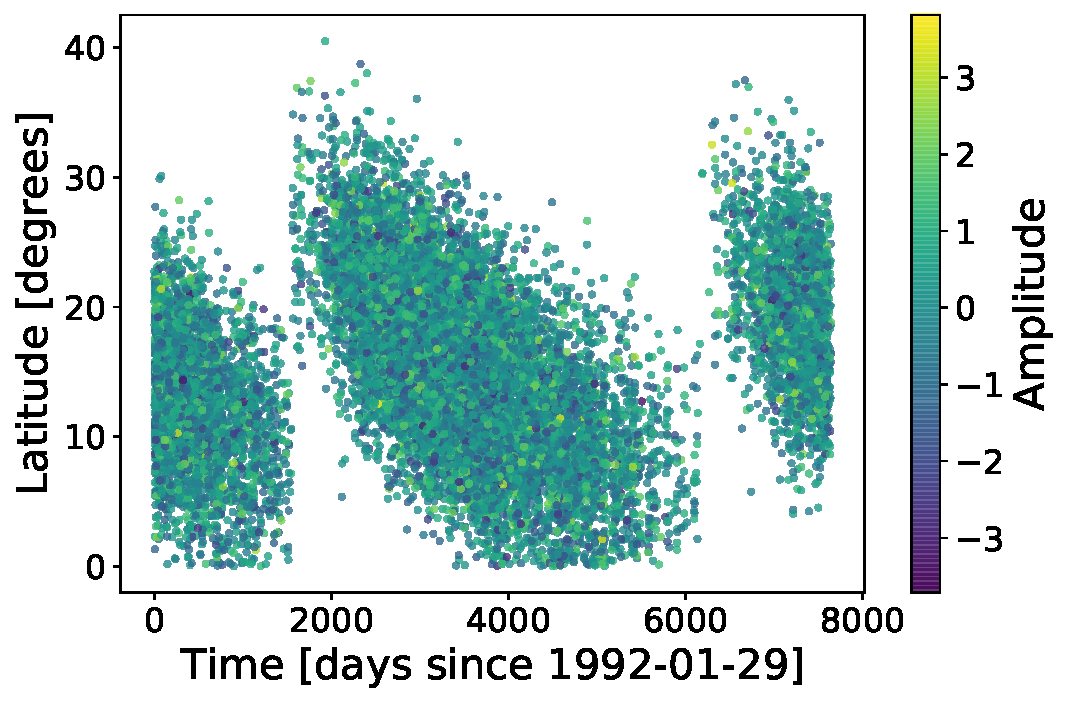
\includegraphics[width=0.85\columnwidth]{24h_fake_butterfly.pdf}
	\caption{Artificial butterfly diagram generated from the simulations, allowing for the parameters to be drawn from distribution to add stochasticity into the simulation.}
	\label{fig:fake_butterfly}
\end{figure}


The resultant power spectra for the two different models (`cosine' and `sign change') show different features, which can be seen in Fig.~\ref{fig:artificial_LS}. These limit spectra were made by combining 100 realisations of the power spectrum. Each individual power spectrum was made using only a single source starting at $t_0 = 0$, and allowing only the phase to vary between the different realisations.

It is clear that the `cosine' model produces a strong peak at the rotational period in the simulation, and a harmonic peak at twice that frequency. This model also produces a significant amount of power at low frequency due to the non-zero mean of the simulated time series. 

On the other hand, the `sign change' model has near-zero low frequency power due to the $\sim$zero mean of the time series. The `sign change' model also produces a strong peak at half the period of rotation in the simulation. There is a smaller peak at the rotational period and at a harmonic of the rotation of 3 times the period.


\begin{figure}[ht!]
	\centering
	\subfloat[`cosine' model \label{fig:cosine_LS}]{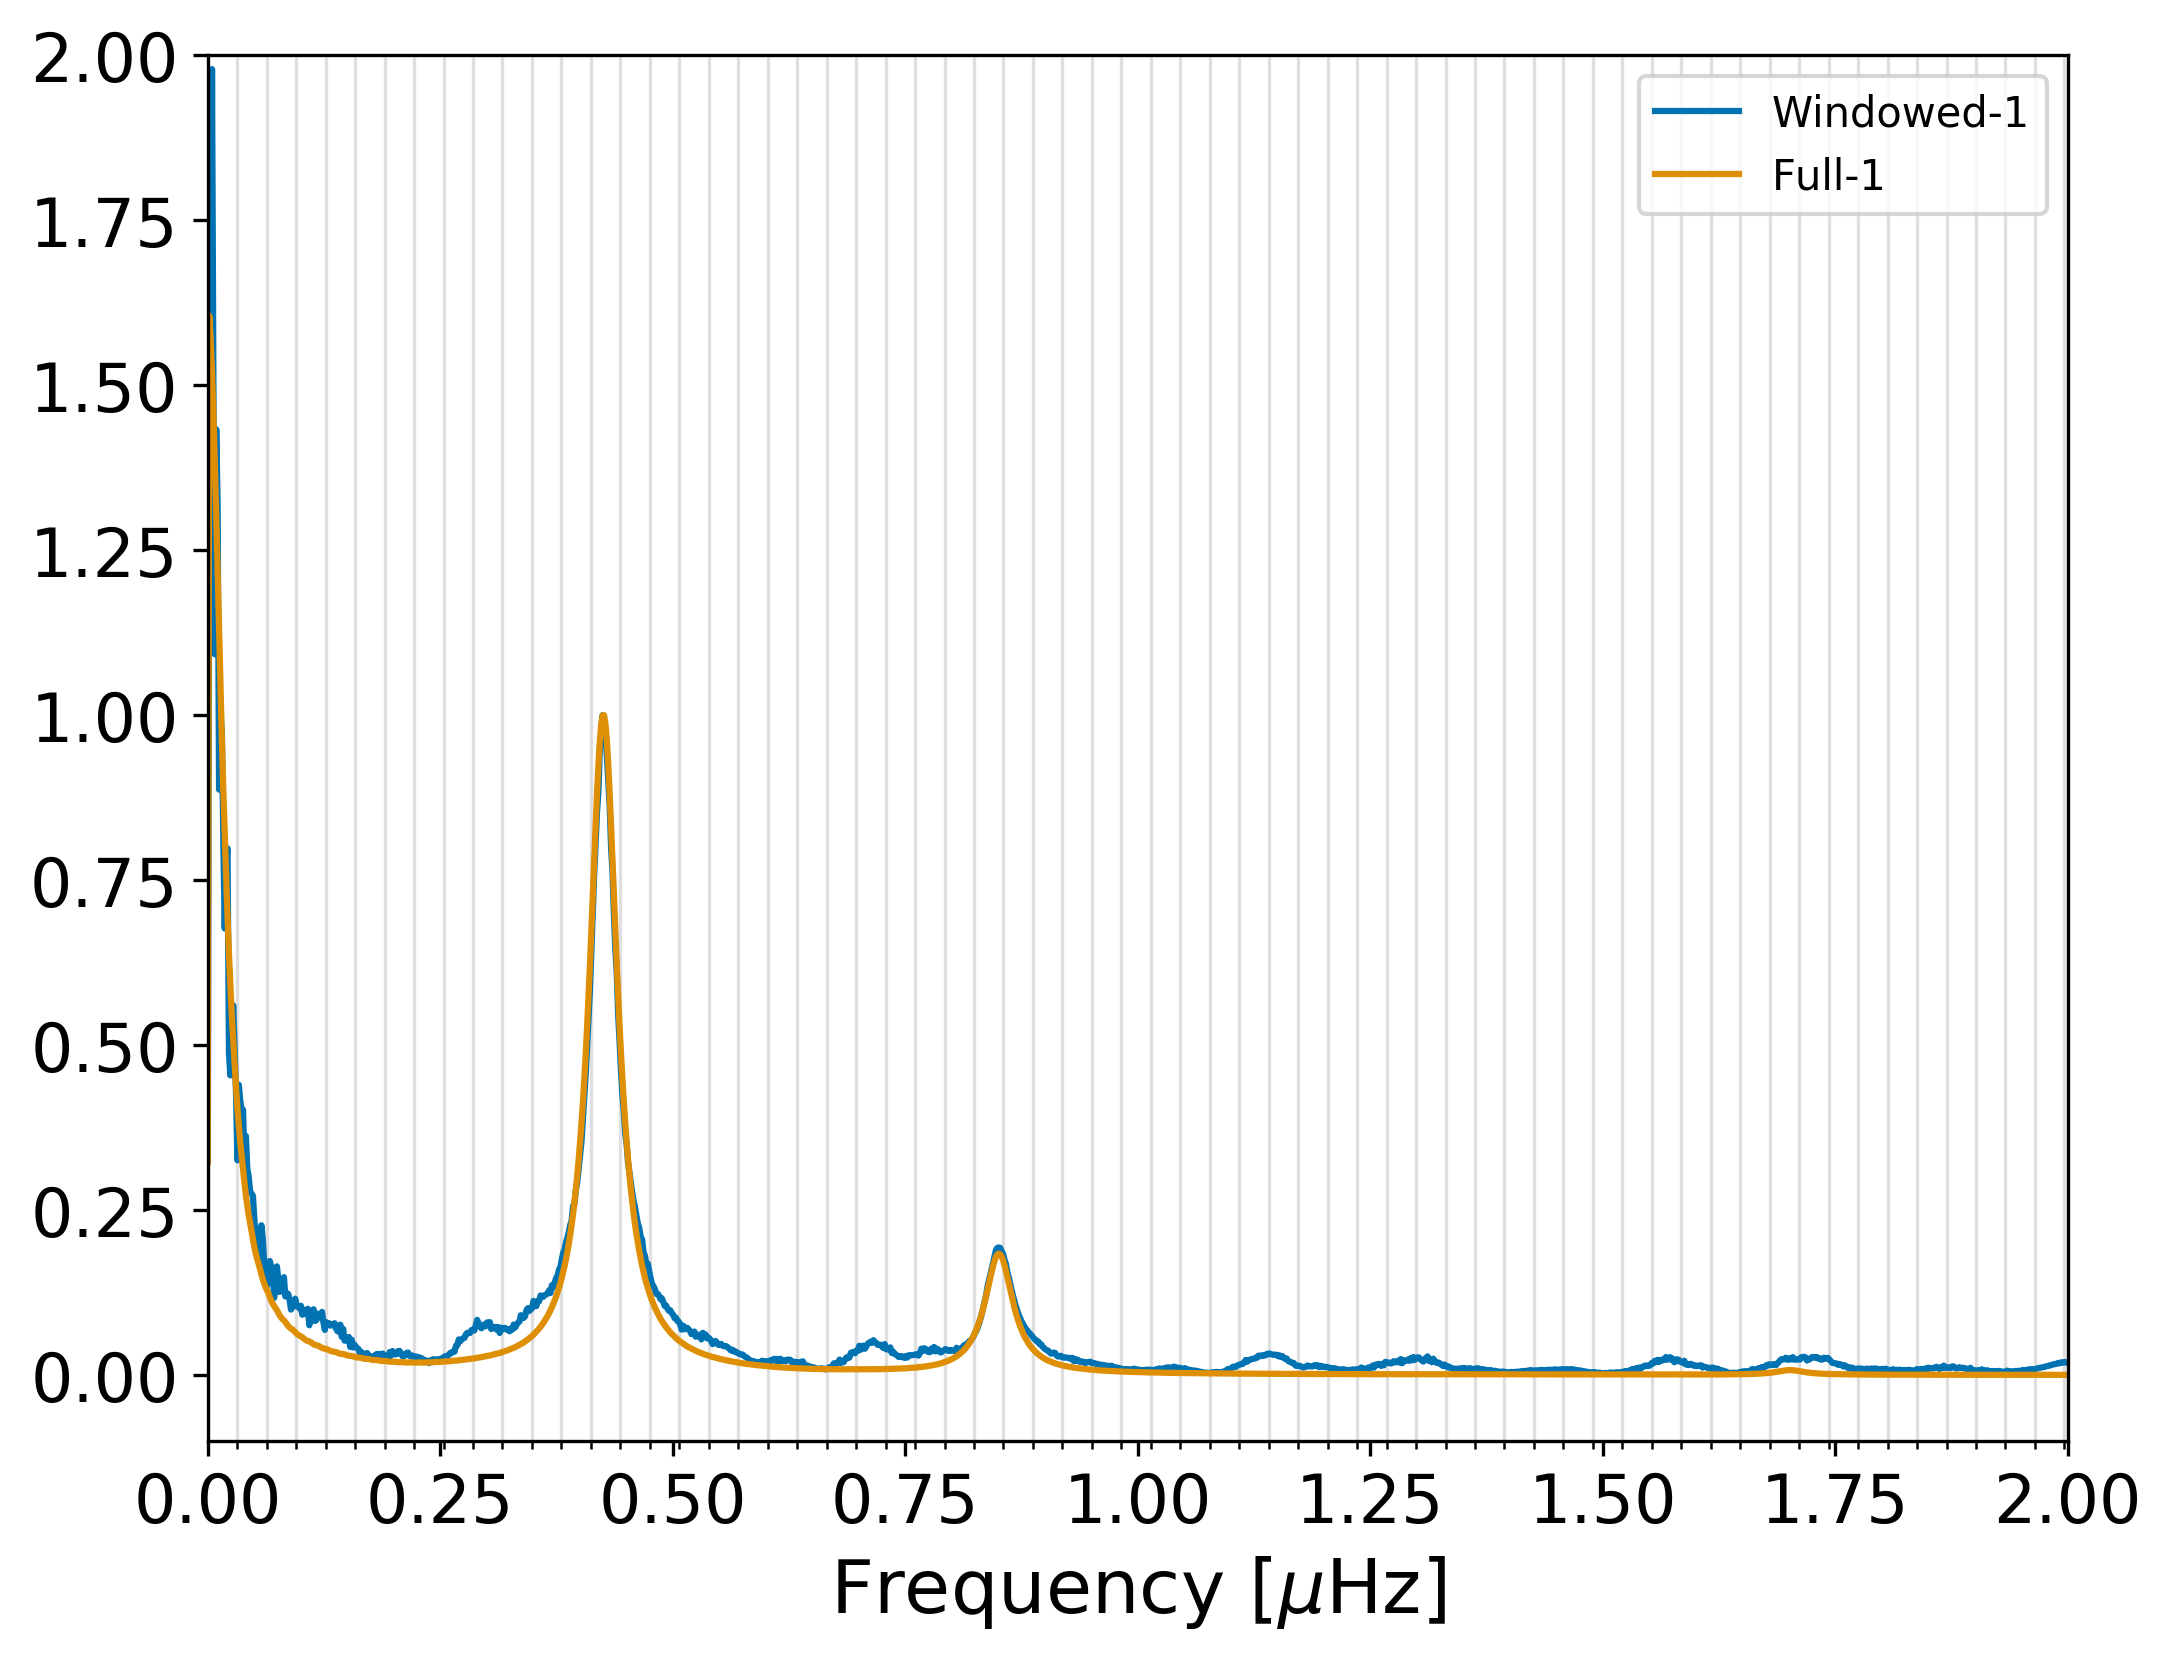
\includegraphics[width=0.45\columnwidth]{cosine_LS.png}} 
	\qquad
	\subfloat[`sign change' model \label{fig:sgn_cng_LS}]{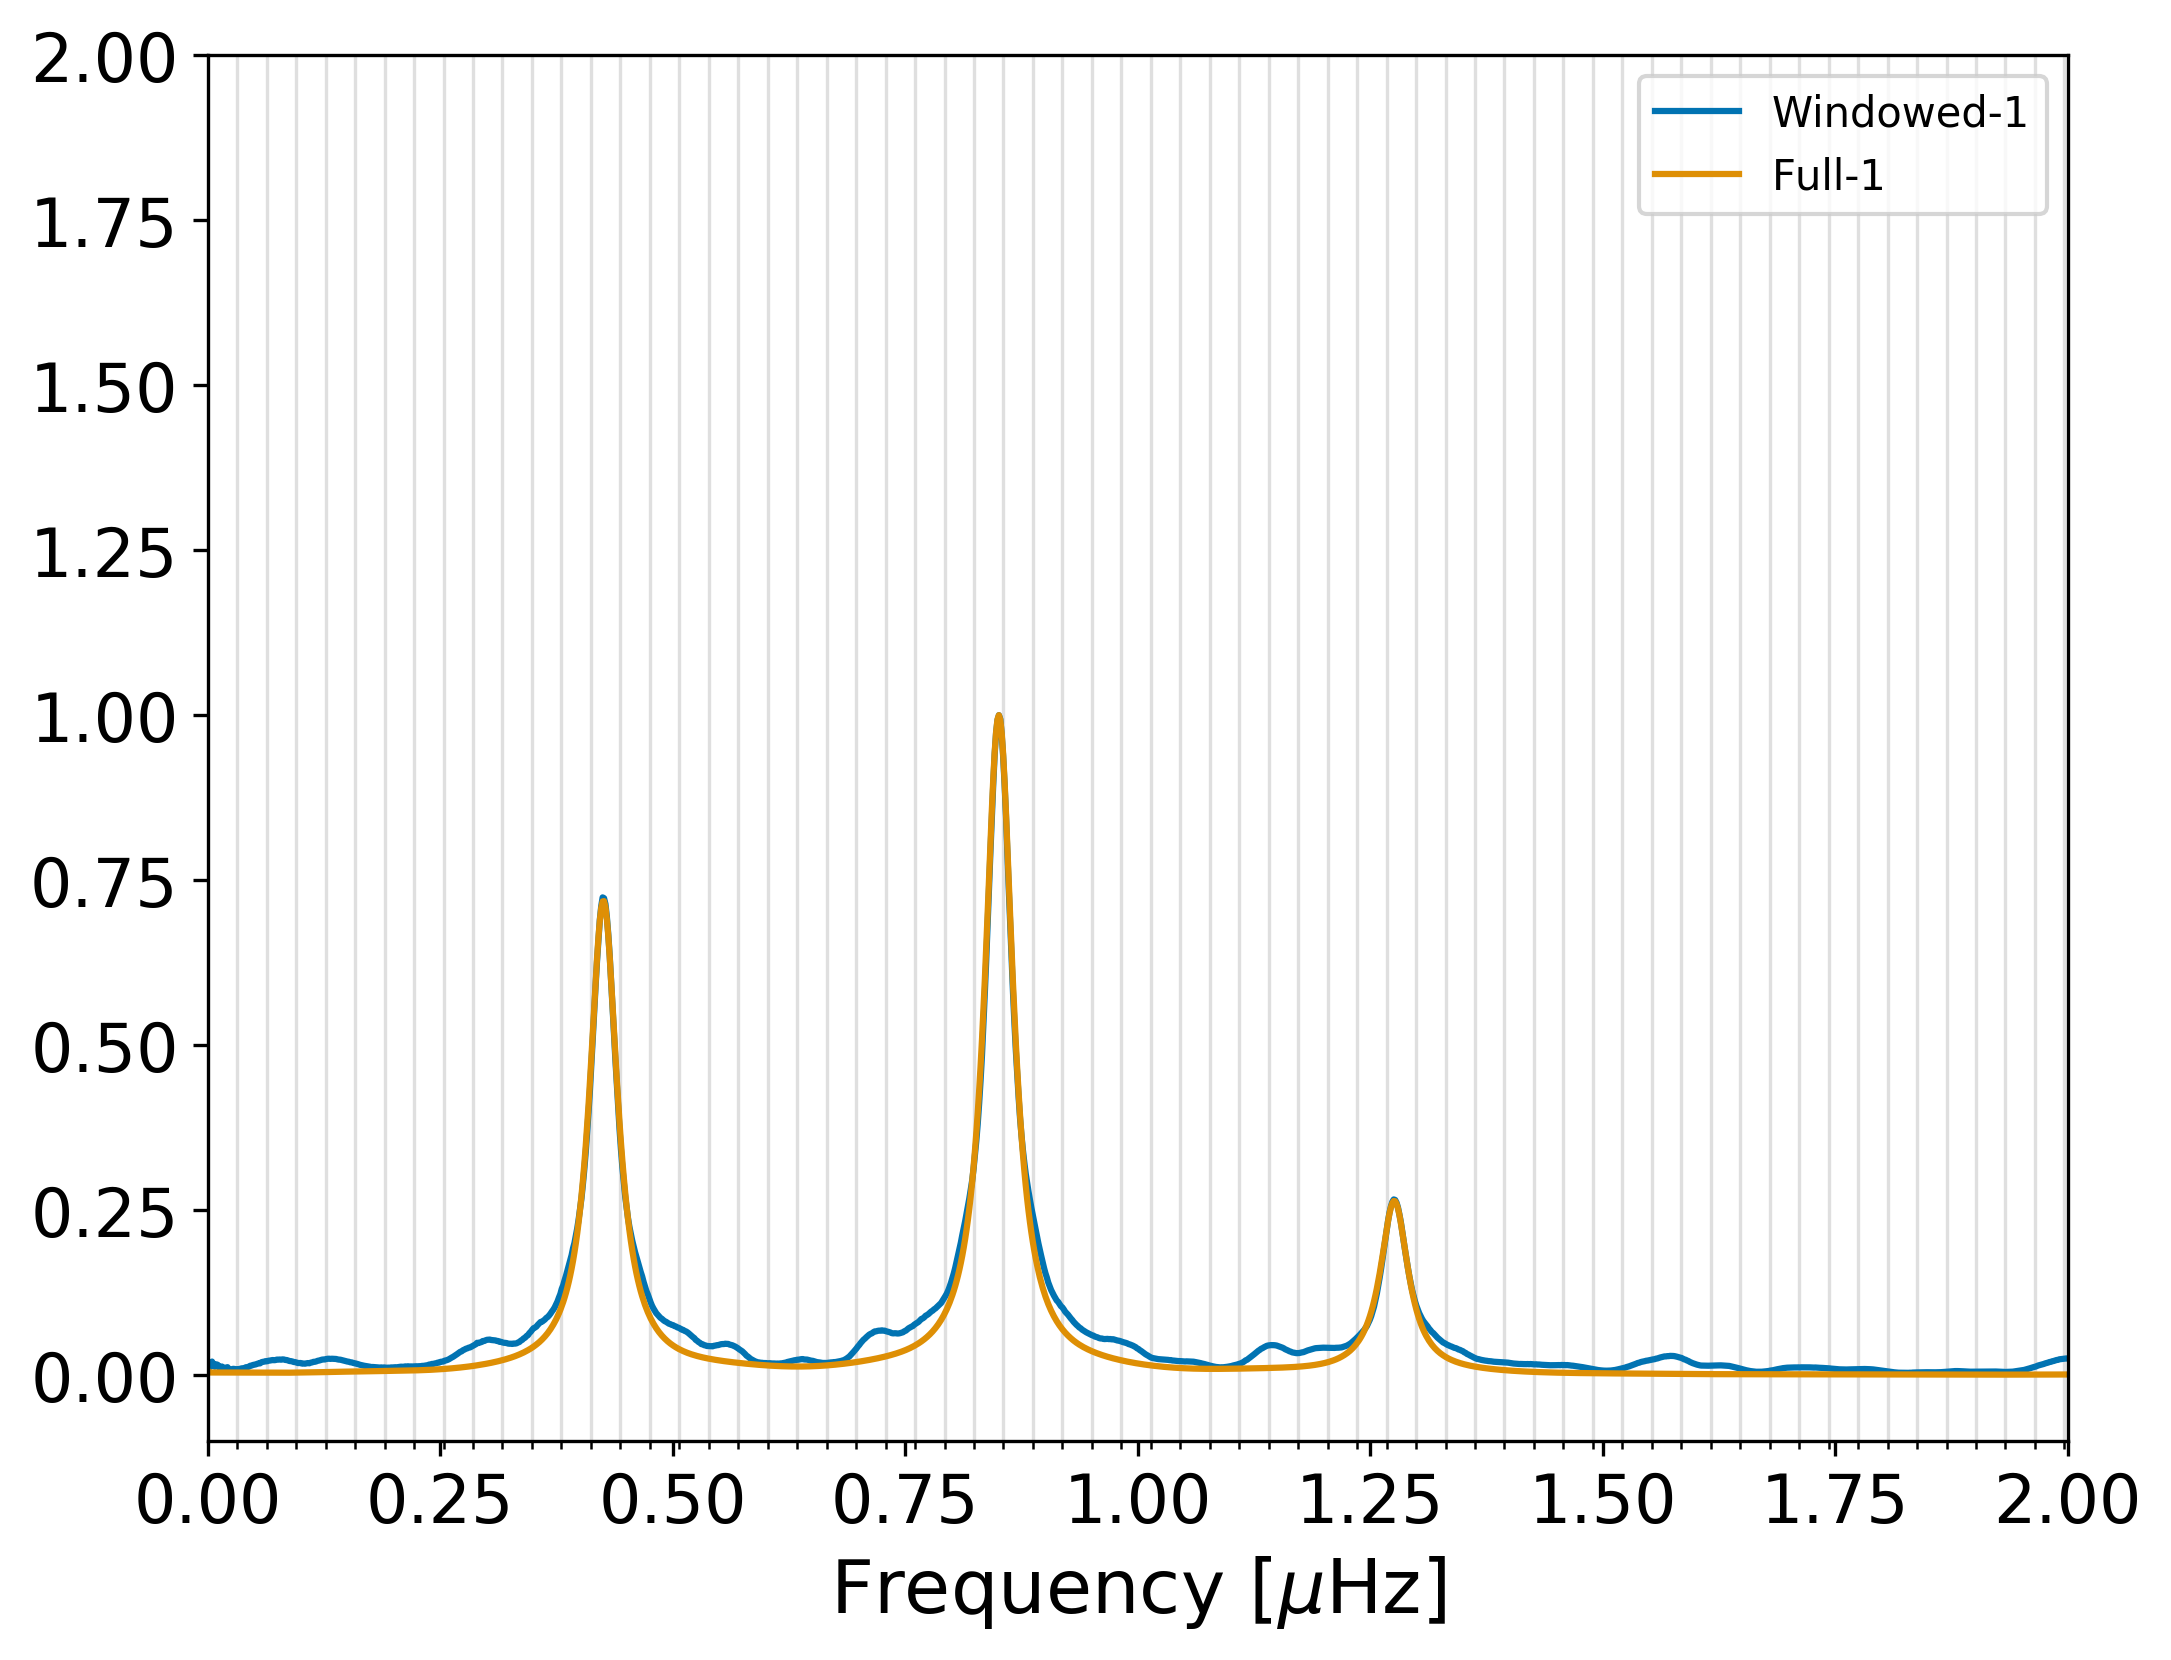
\includegraphics[width=0.45\columnwidth]{sign_change_LS.png}}
	\caption{Limit spectrum from 100 realisations of the cosine model (a) and the sign change model (b) using a single source in each model.}  \label{fig:artificial_LS}
\end{figure}

[include a plot of the comparison between the BiSON PSD and the artificla PSDs -- is it also worth showing the time series...? probably!]

